%\documentclass[a4paper,11pt]{article}

%\documentclass{article}

%\begin{document}

\documentclass[12pt]{article}
\usepackage{latexsym,multicol,graphicx,rotating}
\usepackage[utf8]{inputenc}
\usepackage[sorting=none, style = numeric]{biblatex}
%\usepackage[sorting=none, style = science]{biblatex}
\addbibresource{references.bib}
\usepackage{graphicx}
%\usepackage{authblk}
\usepackage[margin=1 in]{geometry}
\usepackage{amsmath}
\usepackage[font=small, margin=1 in]{caption}

%Peter
\usepackage{easylist}
\newcommand{\bl}{\begin{easylist}}
\newcommand{\el}{\end{easylist}}
\usepackage{todonotes}
\presetkeys{todonotes}{inline,color=blue!30, size=\small}{}
%\newcommand{\nexp}{PiENuXe}
\newcommand{\nexp}{PIENUX}
\newcommand{\ssp}{\vspace{1mm}}

%\usepackage{amsmath}
%\usepackage{amssymb}
%\usepackage{dcolumn}
%\usepackage{longtable}
%\usepackage{pifont}

% Use Michel Goossens' dense lists Itemize, Enumerate and Description

\let\Otemize =\itemize
\let\Onumerate =\enumerate
\let\Oescription =\description
% Zero the vertical spacing parameters
\def\Nospacing{\itemsep=0pt\topsep=0pt\partopsep=0pt\parskip=0pt\parsep=0pt}
% Redefine the environments in terms of the original values
\newenvironment{Itemize}{\Otemize\Nospacing}{\endlist}
\newenvironment{Enumerate}{\Onumerate\Nospacing}{\endlist}
\newenvironment{Description}{\Oescription\Nospacing}{\endlist}

\newcounter{expnum}

\renewcommand{\thebibliography}[1]{\list
 {\arabic{enumi}.}{\settowidth\labelwidth{[#1]}\leftmargin\labelwidth
 \advance\leftmargin\labelsep
 \usecounter{enumi}}
 \renewcommand{\newblock}{\hskip .11em plus .33em minus -.07em}
 \itemsep=0pt\topsep=0pt\partopsep=0pt\parskip=0pt\parsep=0pt
 \sloppy
 \sfcode`\.=1000\relax}
\let\endthebibliography=\endlist

\makeatletter
\renewcommand{\ps@plain}{%
 \renewcommand{\@oddhead}{\sffamily\bfseries
 \hspace{-2mm}%
 \begin{tabular}[t]{|p{180mm}|}\hline
  {\footnotesize
  TRIUMF EEC New Letter of Intent
  \hspace{\fill}
  Detailed Statement of Proposed Research for Experiment \#: \theexpnum}\\ \hline
 \rule[-242mm]{0mm}{0mm}\\ \hline
 \end{tabular}}
 \renewcommand{\@evenhead}{\@oddhead}
 \renewcommand{\@oddfoot}{\sffamily\hfil\thepage\hfil}
 \renewcommand{\@evenfoot}{\@oddfoot}}
\makeatother
\textwidth      180mm
\textheight     240mm
\topmargin      -20mm
\oddsidemargin   -7mm
\flushbottom
\frenchspacing

\pagestyle{plain}

\begin{document}

\setcounter{expnum}{2127}
%{S2127LOI}

\title{TRIUMF S2127LOI: Rare Pion Decay }

\date{March 29, 2021}





\maketitle

%\tableofcontents
%\abstract{

A next-generation rare pion decay experiment is strongly motivated by several inconsistencies between Standard Model (SM) predictions and data pointing towards the violation of lepton flavor universality. It can probe non-SM explanations of these anomalies due to sensitivity to quantum effects of new particles even if their masses are at a very high scale.
Using state-of-the-art instrumentation, computational resources, and a new high-intensity beam, the experiments can be performed at TRIUMF.
%with nearly the same apparatus and beamline. 
Measurement of the charged-pion branching ratio to electrons vs.\ muons $R_{e/\mu}$ is extremely sensitive to a wide variety of new physics effects. At present, the SM prediction for $R_{e/\mu}$ is known to 2 parts in $10^4$, which is 15 times more precise than the current experimental result.  An experiment at a comparable level of accuracy allows a  test of lepton flavor universality at an unprecedented level, probing mass scales up to 3000 TeV. Measurement of  the rare process of pion beta decay, $\pi^+\to \pi^0 e^+ \nu (\gamma)$) with an order of magnitude improvement in sensitivity will determine $V_{ud}$ in a theoretically pristine manner and test CKM unitarity at the quantum loop level. In addition, various exotic rare decays involving e.g.\ sterile neutrinos and  axions will be searched for with unprecedented sensitivity.  The experiment design benefits from experience with the recent PIENU and PEN efforts at TRIUMF and PSI.  Improved resolution, greatly increased calorimeter depth, high-speed detector and electronic response, large solid angle coverage, and complete event reconstruction   are all critical to the new approach which includes  a 3$\pi$ sr 30 radiation length  calorimeter, a segmented active stopping target, and an electron tracker, as well as a new customized pion production target and pion beam line.   }

\section{Scientific Value}


%\section{Theory}
%\subsection{$\boldsymbol{R_{e/\mu}}$ and lepton flavor universality}

The branching ratio 
%\begin{equation}
$R_{e/\mu} = \frac{\Gamma\left(\pi^+ \rightarrow e^+ \nu (\gamma) \right)}{\Gamma\left(\pi^+ \rightarrow \mu^+ \nu (\gamma)\right)}$
%\end{equation}
for pion decays to electrons over muons provides the best test of electron--muon universality in charged-current weak interactions. In the Standard Model (SM), $R_{e/\mu}$ has been calculated with extraordinary precision at the $10^{-4}$ level as \cite{Cirigliano1,Cirigliano2,Bryman1}
\begin{equation}
\label{Remu_SM}
    R_{e/\mu} \hspace{0.1cm}\text{(SM)} = (1.2352\pm 0.0002)\times10^{-4},
\end{equation}
perhaps the most precisely calculated weak interaction observable involving quarks. Because the
uncertainty of the SM calculation for $R_{e/\mu}$ is very small and the decay $\pi^+ \rightarrow e^+ \nu$ is helicity-suppressed by the $V-A$ structure of charged currents, a measurement of $R_{e/\mu}$ is extremely sensitive to the presence of pseudo-scalar (and scalar) couplings absent from the SM; a disagreement with the theoretical expectation would unambiguously imply the existence of new physics beyond the SM. With measurements of 0.01\% experimental precision, new physics beyond the SM (BSM) up to the mass scale of 3000 TeV may be revealed by a deviation from the precise SM expectation \cite{Bryman1}. Possible sources of deviation include new interactions involving scalar particles like Majorons \cite{Lessa}, charged Higgs particles, and leptoquarks \cite{Campbell}. Supersymmetry models with and without $R$-parity violation \cite{Ramsey-Musolf} or with lepton flavor violating terms \cite{Masiero} could also cause deviations from the SM prediction. Other new physics effects which could modify $R_{e/\mu}$ include massive sterile neutrinos \cite{Bryman2} and dark sector processes such as $\pi^+ \rightarrow e^+ \nu \hspace{1mm}\textrm{X}$ \cite{Altmannshofer}, which are also sought in the rare pion decay experiments \cite{Aguilar-Arevalo1, Aguilar-Arevalo2}. 

\paragraph{}
Currently, the most accurate measurement was reported by PIENU \cite{Aguilar-Arevalo3},
\begin{equation}
\label{Remu_exp}
     R_{e/\mu} \hspace{0.1cm} \text{(Expt)} = (1.2344 \pm 0.0023 (\text{stat}) \pm 0.0019 (\text{syst})) \times 10^{-4},
\end{equation}
 at the 0.2\%  precision level. It corresponds to a test of $e$--$\mu$ universality $g_e/g_\mu = 0.9996 \pm 0.0012$, expressed as the ratio of potentially distinct weak couplings for the electron and muon. The result is in excellent agreement with the SM expectation in contrast to recent hints of violation of third generation lepton flavor universality in some $B$-meson decays \cite{LFVB}. The goals of the present TRIUMF PIENU \cite{Aguilar-Arevalo4, Aguilar-Arevalo5} and PSI PEN \cite{Pocanic1, Pocanic2, Pocanic3} experiments are to improve the measurement precision by another factor of 2 or more to a level of $<0.1\%$. However, even if these goals are realized, this still leaves room for experimental improvement by more than an order of magnitude in uncertainty to confront
the SM prediction and to search for BSM effects. The goal of a future experiment discussed below would be a further improvement in precision by an order of magnitude to 0.01\%, making the
experimental uncertainty comparable to the theoretical uncertainty.

%\subsection{Pion beta decay}


\begin{figure}[t!]
\centering
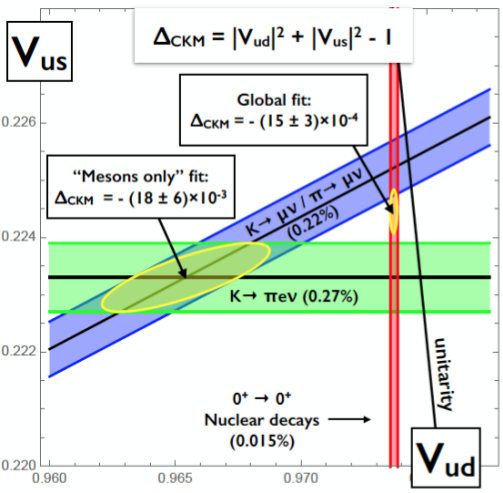
\includegraphics[scale=0.5]{sections/figures/fig-ckm.png}
\caption{Existing tensions in the 1st-row CKM unitarity test.}
\label{fig:CKM}
\end{figure}


The uncertainty of the SM prediction~\eqref{Remu_SM} for $R_{e/\mu}$ arises from low-energy constants in chiral perturbation theory, which absorb the divergences in the two-loop calculation of Refs.~\cite{Cirigliano1,Cirigliano2}, but whose finite parts need to be determined by other means. Fortunately, in the case of  $R_{e/\mu}$ these nonperturbative uncertainties only affect the SM prediction at the relative precision of $10^{-4}$, more than an order of magnitude beyond the current experimental precision~\eqref{Remu_exp}. $R_{e/\mu}$ thus provides a unique opportunity for a pristine test of lepton flavor universality (LFU) in the quark sector. 

While no particles beyond the ones of the SM have been observed so far at the LHC, experiments have accumulated intriguing hints for the violation of LFU (LFUV) within recent years. In particular, the measurements of the ratios $R(D^{(*)})$~\cite{Lees:2012xj,Aaij:2017deq,Abdesselam:2019dgh} and $R(K^{(*)})$~\cite{Aaij:2017vbb,Aaij:2019wad} deviate from the SM expectation of LFU by more than $3\sigma$~\cite{Amhis:2019ckw,Murgui:2019czp,Shi:2019gxi,Blanke:2019qrx,Kumbhakar:2019avh} and $4\sigma$~\cite{Alguero:2019ptt,Aebischer:2019mlg,Ciuchini:2019usw,Arbey:2019duh}, respectively. In addition, the anomalous magnetic moments $(g-2)_\ell$ of charged leptons also measure the violation of LFU as they vanish in the massless limit. Here, there is the long-standing discrepancy in $(g-2)_\mu$ of about $3.7\sigma$~\cite{Bennett:2006fi,Aoyama:2020ynm}. In addition, there is a $2\sigma$ tension in $\tau\to\mu\nu\nu/\tau\to e\nu\nu$~\cite{Aoki:2019cca}, and also the deficit in first-row CKM unitarity shown in Fig.~\ref{fig:CKM}  can be viewed as a sign of LFUV~\cite{Crivellin:2020lzu}. 

\begin{figure}[t!]
\centering
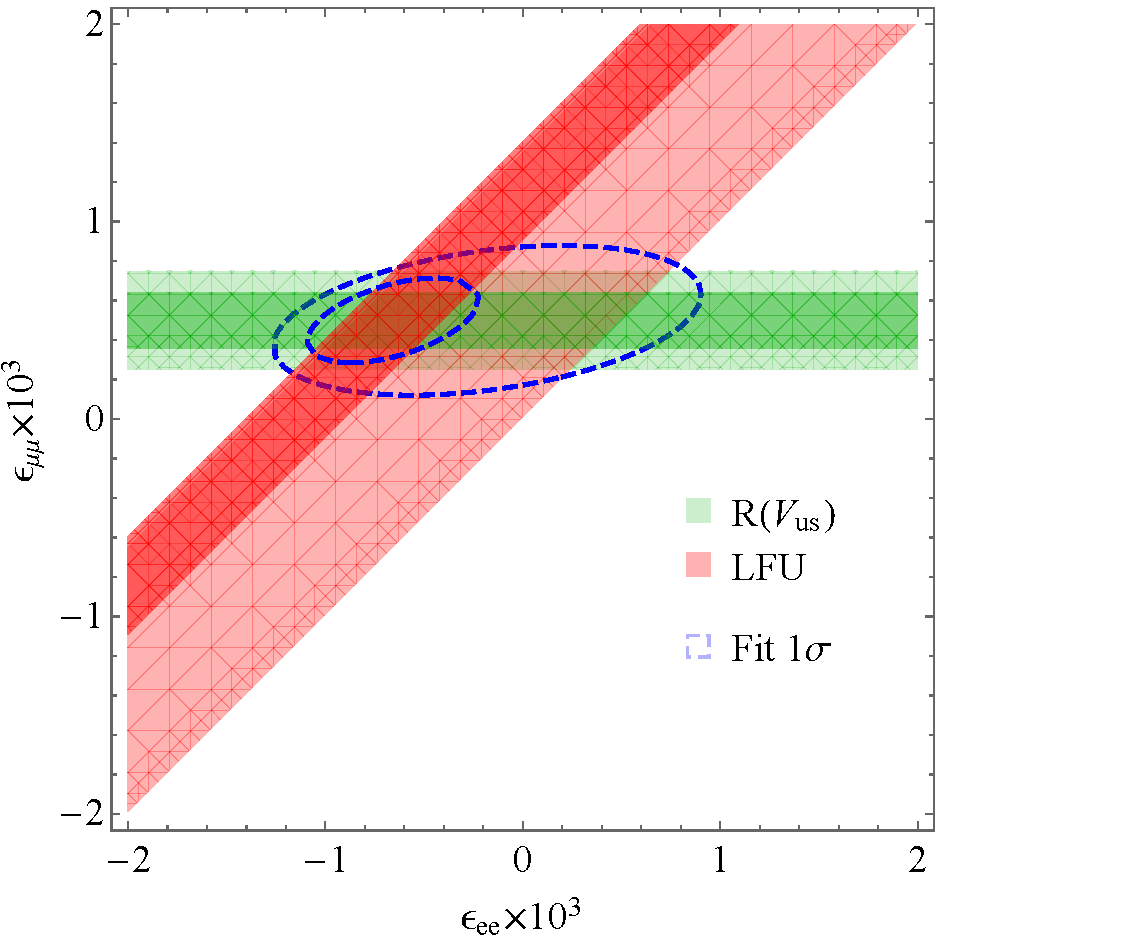
\includegraphics[scale=0.5]{sections/figures/Fit.pdf}
\caption{Modifications of the $W\ell\nu$ couplings, parameterized according to $\delta_{ij}+\epsilon_{ij}$~\cite{Crivellin:2020lzu}. The green bands refer to the constraint from $V_{ud}$ and $V_{us}$ via nuclear $\beta$ decays and kaon decays, the red band to other tests of LFU, dominated by $R_{e/\mu}$ and $\tau\to\mu\nu\nu/\tau\to e\nu\nu$. The light bands refer to the present situation, the dark ones to future projections.}
\label{fig:Fit_epsii}
\end{figure}

For the latter,  assuming that LFUV  originates from modified $W\ell\nu$ couplings, mainly the determination from $\beta$ decays is affected, due to a CKM enhancement by $(V_{ud} / V_{us})^2 \sim 20$. If this effect is real, and corrected for, the red band in Fig.~\ref{fig:CKM} will move to the left. Such a modification of the $W\ell\nu$ couplings would also affect $R_{e/\mu}$, albeit for a different flavor combination, see Fig.~\ref{fig:Fit_epsii}. 
In fact, this connection provides further motivation for the current proposal, especially because the sensitivity to LFUV would be comparable to future improved constraints from $\beta$ decays. Moreover, recent global fits to electroweak observables and tests of LFU show a preference for $R_{e/\mu}$ bigger than its SM expectation \cite{Coutinho:2019aiy,Crivellin:2020ebi}.









%\subsection{Pion beta decay}

The detector optimized for a next-gen $R_{e/\mu}$ experiment will also be ideally suited for a high-precision measurement of pion beta decay and searches for exotic pion and muon decays. Precision measurements of beta decays of neutrons,
nuclei, and mesons provide very accurate determinations of the elements $|V_{ud}|$ and $|V_{us}|$ of the
Cabibbo-Kobayashi-Maskawa (CKM) quark-mixing matrix \cite{Cabibbo, Kobayashi}. Recent theoretical
developments on radiative corrections and form factors have led to a $3\sigma$ tension with CKM
unitarity illustrated in Fig.~\ref{fig:CKM}, which, if confirmed, would point to new physics in the multi-TeV scale (see, e.g., Ref.~\cite{Czarnecki}).  
Pion beta decay, $\pi^+ \rightarrow \pi^0 e^+ \nu (\gamma)$, provides the theoretically cleanest determination of the CKM matrix element $V_{ud}$. With current input one obtains $V_{ud} = 0.9739(28)_{\textrm{exp}}(1)_{\textrm{th}}$, where the experimental uncertainty comes almost entirely from the  $\pi^+ \rightarrow \pi^0 e^+ \nu (\gamma)$ branching ratio (BRPB) \cite{Pocanic4} (pion lifetime contributes ${\delta}V_{ud} = 0.0001$), and the theory uncertainty has been reduced from $({\delta}V_{ud})_{\textrm{th}} = 0.0005$ \cite{Sirlin, Cirigliano3, Passera} to $({\delta}V_{ud})_{\textrm{th}} = 0.0001$ via a lattice QCD calculation of the radiative corrections \cite{Feng}. The current precision of 0.3\% on $V_{ud}$ makes $\pi^+ \rightarrow \pi^0 e^+ \nu (\gamma)$ not presently relevant for the CKM unitarity tests because super-allowed nuclear beta decays provide a nominal precision of %0.015\%. 
0.03\%. 



In order to make $\pi^+ \rightarrow \pi^0 e^+ \nu (\gamma)$ important for CKM unitarity tests, two precision experimental stages can be identified:
%\begin{enumerate}  
(1) As advocated in Ref.~\cite{Czarnecki}, a three-fold improvement in BRPB precision compared to Ref.~\cite{Pocanic3} would allow for a 0.2\% determination of $V_{us}/V_{ud}$ improving on measurement of  the ratio currently 
 %   \begin{equation}
      $  R_V = \frac{\Gamma\left(\textrm{K} \rightarrow \pi l \nu (\gamma) \right)}{\Gamma\left(\pi^+ \rightarrow \pi^0 e^+ \nu (\gamma)\right)}=1.3367(25)$ ,
 %   \end{equation}
    independent of the Fermi constant, short-distance, and structure-dependent radiative corrections. This
    would match the precision of the current extraction of $V_{us} / V_{ud}$ from the axial channels~\cite{Marciano} by making improvements to the current 
  % \begin{equation}
        $R_A = \frac{\Gamma\left(\textrm{K} \rightarrow \mu \nu (\gamma) \right)}{\Gamma\left(\pi \rightarrow \mu \nu (\gamma)\right)}=1.9884(115)(42)$,
 %   \end{equation}
    (see Fig. \ref{fig:CKM}), thus providing a new competitive constraint on the $V_{us}$--$V_{ud}$ plane and probing new physics that might affect vector and axial-vector channels in different ways.
    The theoretical case for this approach was recently strengthened by improved analysis of radiative corrections in $K \to \pi e \nu $ decays \cite{Seng:2021}.  
(2)  In the second phase, an order of magnitude improvement  in the
BRPB precision will be sought. This would provide the theoretically cleanest extraction of $V_{ud}$ at the 0.02\% level. 
%\end{enumerate}

High precision pion decay experiments can access rare and exotic decays, as  demonstrated by
previous experiments like PIENU. Extensions of the Standard Model postulate the
existence of additional (sterile) neutrinos \cite{nuMSM}\cite{BrymanShrock}. These additional states can potentially explain
the small mass of the SM neutrinos and contribute to the solution of outstanding puzzles like
the nature of dark matter  and early cosmological processes like small scale structure formation \cite{bertoni}.  
Exotic pion and muon decays involving sterile neutrinos  and axions in reactions including $\mu\to e a$\cite{Aguilar-Arevalo6},  $\pi \to l \nu_h$\cite{Aguilar-Arevalo1}\cite{Aguilar-Arevalo2} and $\pi \to l \nu a$\cite{Aguilar-Arevalo8} can provide new information on topical non-SM effects; the experiment proposed here will make improvements in sensitivity to such effects by an order of magnitude or more.


%\subsection{Searches for other rare and exotic decays}\label{Exotics}
High precision pion decay experiments can access rare and exotic decays, as  demonstrated by
previous experiments (see Fig~\ref{fig:decays}) like PIENU. Extensions of the Standard Model postulate the
existence of additional (sterile) neutrinos \cite{nuMSM}\cite{BrymanShrock}. These additional states can potentially explain
the small mass of the Standard Model neutrinos and contribute to the solution of outstanding puzzles like
the nature of dark matter  and early cosmological processes like small scale structure formation \cite{bertoni}.  
Massive neutrino states $\nu_H$ can be sought in the two-body pion decays
$\pi^+\rightarrow e^+\nu_H$ \cite{Aguilar-Arevalo1} and $\pi^+\rightarrow \mu^+\nu_H$ \cite{Aguilar-Arevalo2}. Exploiting
large datasets of pion decays and the resulting decay muons,  exotic two-body muon decays like $\mu^+\rightarrow e^+X$ can
be sought \cite{Aguilar-Arevalo6}, where X is a massive neutral boson (e.g. an axion or a Majoron).
Similarly, exotic particles have been searched for in three body decays like $\pi^+\rightarrow l^+ \nu X$ ($l=e^+,\mu^+$) \cite{Aguilar-Arevalo8}.
The PIENU experiment also obtained upper limits for the rare decays $\pi^+\rightarrow e^+\nu_e\nu\bar{\nu}$ and
$\pi^+\rightarrow \mu^+\nu_{\mu}\nu\bar{\nu}$ at the $10^6-10^7$ level \cite{Aguilar-Arevalo7}.\\
An experiment with two orders of magnitude more statistics has the potential to improve the existing limits by at least an order of magnitude.
Since the searches are based on a fit to the energy spectra of the visible final state particles, an improved experiment
can bring significant additional advantages in lowering the limits and in reducing the systematic errors. For example, 
the $\pi^+\rightarrow e^+\nu$ low energy tail represents a relevant background for the
$\pi\rightarrow e^+\nu_H$, $\pi^+\rightarrow e^+\nu X$, and $\pi^+\rightarrow e^+\nu_e\nu\bar{\nu}$ searches: 
more precise knowledge of the tail and its further reduction will significantly improve the upper limits beyond the statistics.
The search for rare and exotic decays involving  muons, like $\pi^+\rightarrow \mu^+\nu_H$, $\pi^+\rightarrow \mu^+\nu X$, and $\pi^+\rightarrow \mu^+\nu_{\mu}\nu\bar{\nu}$ will
benefit from an improved stopping target and faster electronics, which will allow better separation of  muons from pions and thus further improve the sensitivity.
Taking into account all the characteristics of an improved pion decay experiment, improvements by more than an order of magnitude can be expected.
\begin{figure}
    \centering
    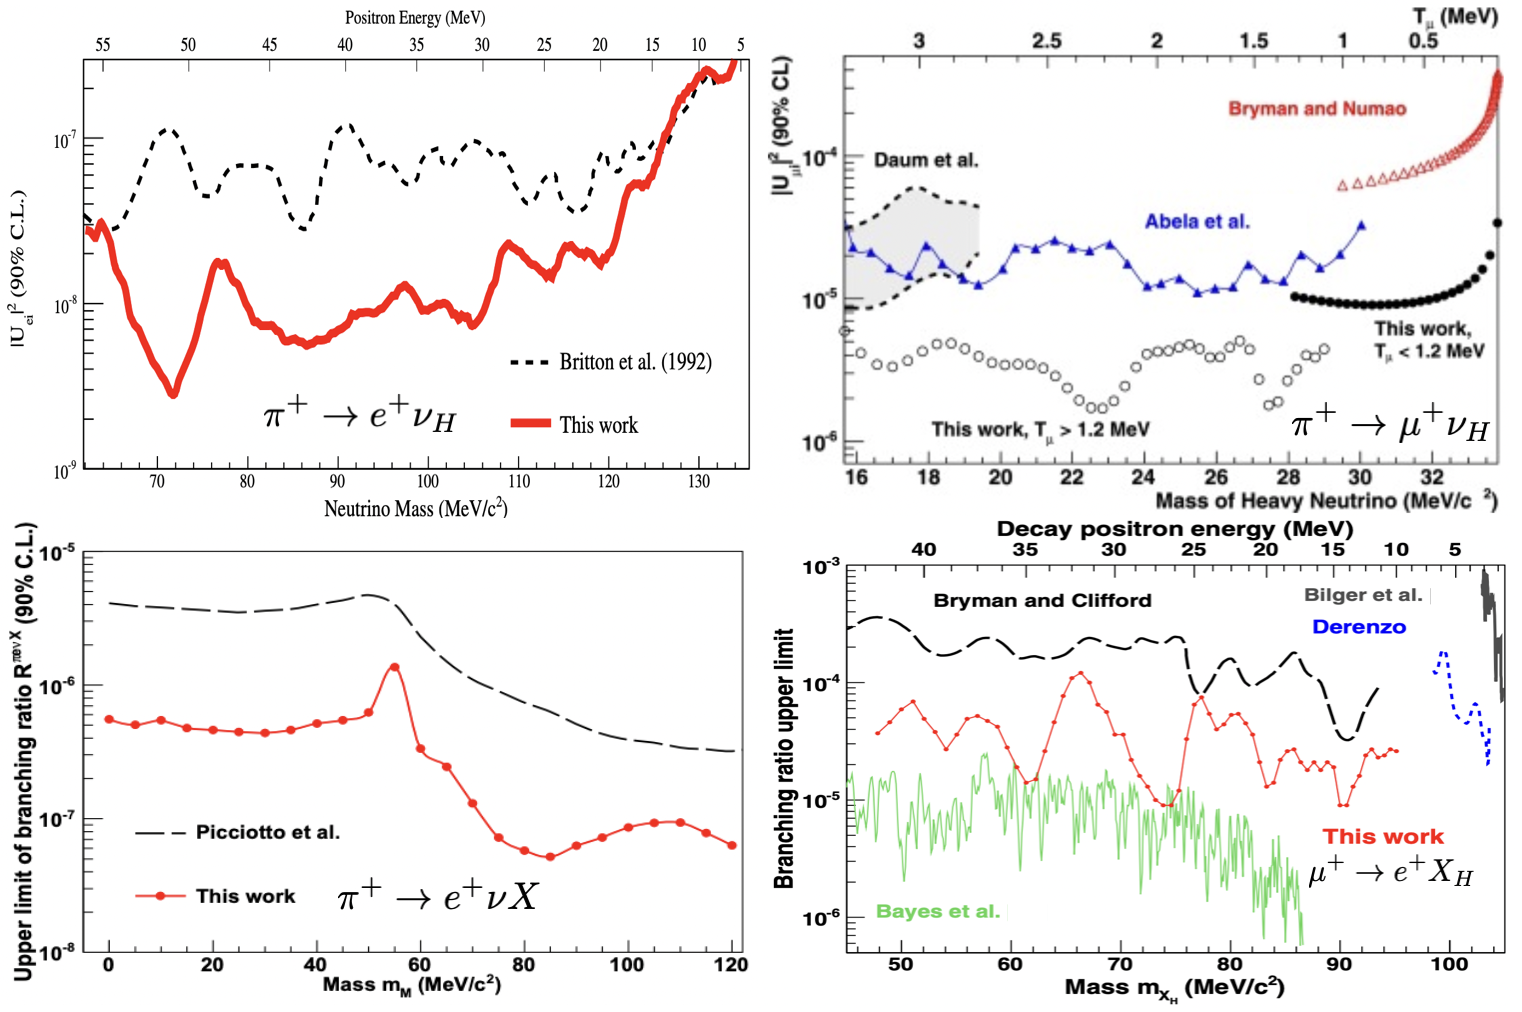
\includegraphics[width=0.6\textwidth]{sections/figures/RareResults.png}
    \caption{Exotic decay searches from the PIENU experiment. The 
    results are indicated with "This work" and show order of magnitude improvements in sensitivity over
    previous experiments.}
    \label{fig:decays}
\end{figure}




%\clearpage
\section{\nexp\ Description of the Experiment}\label{s:PIENUXEdet}
%\subsection{Concepts}
%Precision frontier experiments require very high statistics as well as extensive evaluation of systematic uncertainties, backgrounds, biases and distortions in the data selection criteria. The two experiments, TRIUMF PIENU and PSI PEN  provide highly insightful information on the  limitations of their techniques and the principal systematic effects. We will briefly describe the general characteristics of the decay channels measured as well as discuss the designs adopted by the PIENU and PEN experiments.

The previous measurements were performed using stopped pions that decay at rest either directly to a positron and a neutrino ($\pi^+ \rightarrow e^+ \nu$ decay) or first to a muon (and associated neutrino) that subsequently undergoes 3-body decay at rest in the target (decay chain $\pi^+ \rightarrow \mu^+ \rightarrow e^+$). The  energy and time characteristics of the positrons emerging from those two decays are very different, and thus can be used to distinguish the decay channels. By measuring the ratio of positrons detected from the two channels, many systematic effects (e.g. pion counting, solid angle acceptance, efficiency, etc.) cancel out to first order, aiding in reaching high precision.


Positrons arising from $\pi^+ \rightarrow e^+ \nu$ are monoenergetic giving  69.3 MeV of kinetic energy. The timing distribution is an exponential with the pion lifetime. 
The energy distribution of positrons arising from $\pi^+ \rightarrow \mu^+ \rightarrow e^+$ is the so-called Michel spectrum, extending from 0 to 52.3 MeV of kinetic energy. The timing distribution is the convolution of a pion lifetime and a muon lifetime. Simulated energy and timing distributions for $\pi^+ \to e^+ \nu$ and $\pi^+ \to \mu^+ \to e^+$ events are shown in Fig~\ref{fig:MC_pienu_pimue_time_energy}.

\begin{figure}[h!]
\centering
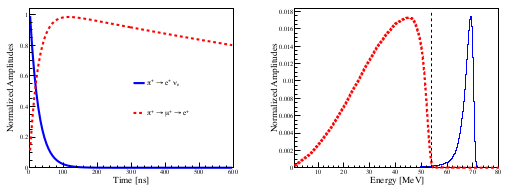
\includegraphics[scale=1.0]{sections/figures/MC_pienu_pimue_time_energy.png}
\caption{Simulated energy (a) and timing (b) distributions for $\pi^+ \to e^+ \nu$ (blue) and $\pi^+ \to \mu^+ \to e^+$ (red) events. }
\label{fig:MC_pienu_pimue_time_energy}
\end{figure}

Since the energy deposited by the decay positrons and their time distributions are important discrimination criteria between the two decay channels,  essential characteristics of the experimental setup  include a high energy resolution calorimeter and fast timing detectors, combined with high frequency, high linearity, signal digitizers.

Muons from  the $\pi^+ \rightarrow \mu^+ \rightarrow e^+$ decay chain deposit $\sim$ 4 MeV in the pion stopping target, which provides an additional handle to discriminate between the two decay modes. The target should thus ideally provide high resolution in energy and cover a large dynamic range to avoid saturation. 
Backgrounds in the time distribution come from decays-in-flight of both pions and muons, necessitating the inclusion of several sets of tracking detectors and a compact detector assembly.

Despite being  mono-energetic the positrons originating from $\pi^+ \rightarrow e^+ \nu$ decays have their energy distribution broadened due to finite energy resolution of the calorimeter, shower leakages of low energy photons from the sides and ends of the calorimeter as well as the presence of radiative decays. Those effects result in a low energy tail hidden under the Michel spectrum and lead to the main correction and largest source of systematic effects in the branching ratio measurement. In order to minimize the energy tail for a precise experiment, a high resolution,  high radiation-length, and high acceptance calorimeter must be chosen.     

%Both experiments used plastic scintillator as the stopping target, and crystal calorimeters for the positron energy measurement. The use of total absorption calorimeters for energy measurements complements the theoretical predictions, which include radiative effects (i.e. $\pi^+ \rightarrow e^+ \nu \gamma$ and $\pi^+ \rightarrow \mu^+ \nu \overline{\nu} \gamma$ decays).
%\subsection{Methods}
%\input {sections/Concepts/methods.tex}

%\subsection{Previous Experiments}
%\subsection{TRIUMF PIENU}
%TRIUMF has a long history of pion branching ratio measurements \cite{Bryman3, Britton}. Each generation of experiment benefited from experience gained during the previous experiment as well as from advances in technology. The experiment that preceded PIENU was performed at TRIUMF in the 1980s and measured the branching ratio to be $(1.2265 \pm 0.0056) \times 10^{-4}$ based on $10^5$ $\pi \to e \nu$ events; the precision was dominated by systematic uncertainties.  PIENU \cite{Aguilar-Arevalo1, Aguilar-Arevalo2, Aguilar-Arevalo4, Aguilar-Arevalo5} accumulated $10^7$ $\pi \to e \nu$ events using an increased solid angle and higher resolution calorimeter, longer running time, and improvements designed to reduce systematic uncertainties. It  reported an interim result at the $0.2\%$ level given in Eq.\ref{Remu_exp} and expects to achieve $0.1\%$ precision.

The largest sources of uncertainty in these experiments have been statistics and the systematic uncertainty related to the low-energy tail correction. The statistical uncertainty for the current PIENU experiment is projected to improve by about a factor of four compared to Ref. \cite{Britton}. 
PIENU used a high-resolution ($\sigma=1\%$) crystal calorimeter consisting of a single NaI(Tl) crystal surrounded by an array of 97 pure CsI crystals. The PIENU detector is shown in Figure~\ref{fig:detector_PIENU} and described in \cite{Aguilar-Arevalo4}. The NaI crystal was 19 radiation lengths thick for on-axis decays.

\begin{figure}[h!]
\centering
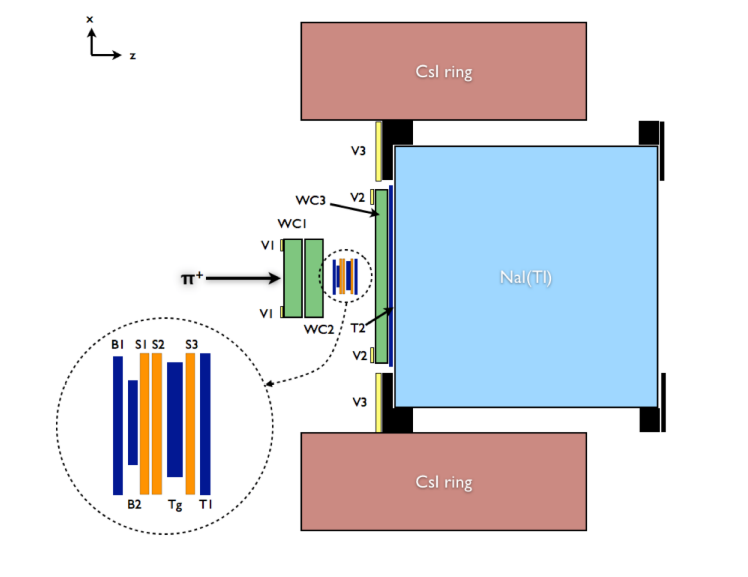
\includegraphics[scale=0.45]{sections/figures/PIENUDetector.png}
\caption{PIENU detector. Plastic scintillators are shown in dark blue, wire chambers in green, silicon strip trackers in orange, and the calorimeter in light blue and red.}
\label{fig:detector_PIENU}
\end{figure}

 PIENU obtained the branching ratio by first separating events into high- and low-energy regions at an energy cut value ($E_{cut}$) as illustrated in Fig. \ref{fig:analysis}. The time spectra were fit in each region with the $\pi^+ \rightarrow e^+ \nu$ and $\pi^+ \rightarrow \mu^+ \rightarrow e^+$ shapes, plus backgrounds originating from different sources including pion decays in flight, contamination from old muon decays etc. The raw branching ratio $R^{raw}_{e/\mu}$ was the ratio of the $\pi^+ \rightarrow e^+ \nu$ amplitude to the $\pi^+ \rightarrow \mu^+ \rightarrow e^+$ amplitude, to which corrections were subsequently applied. %By far the largest correction is the %%%%%, the most significant correction to the raw branching ratioso-called tail correction, which %%%, the most significant correction to the raw branching ratioaccounts for $\pi^+ \rightarrow e^+ %%, the most significant correction to the raw branching ratio\nu$ events with measured energy %%%, the most significant correction to the raw branching ratiobelow $E_{cut}$. 
 
\begin{figure}[h!]
\centering
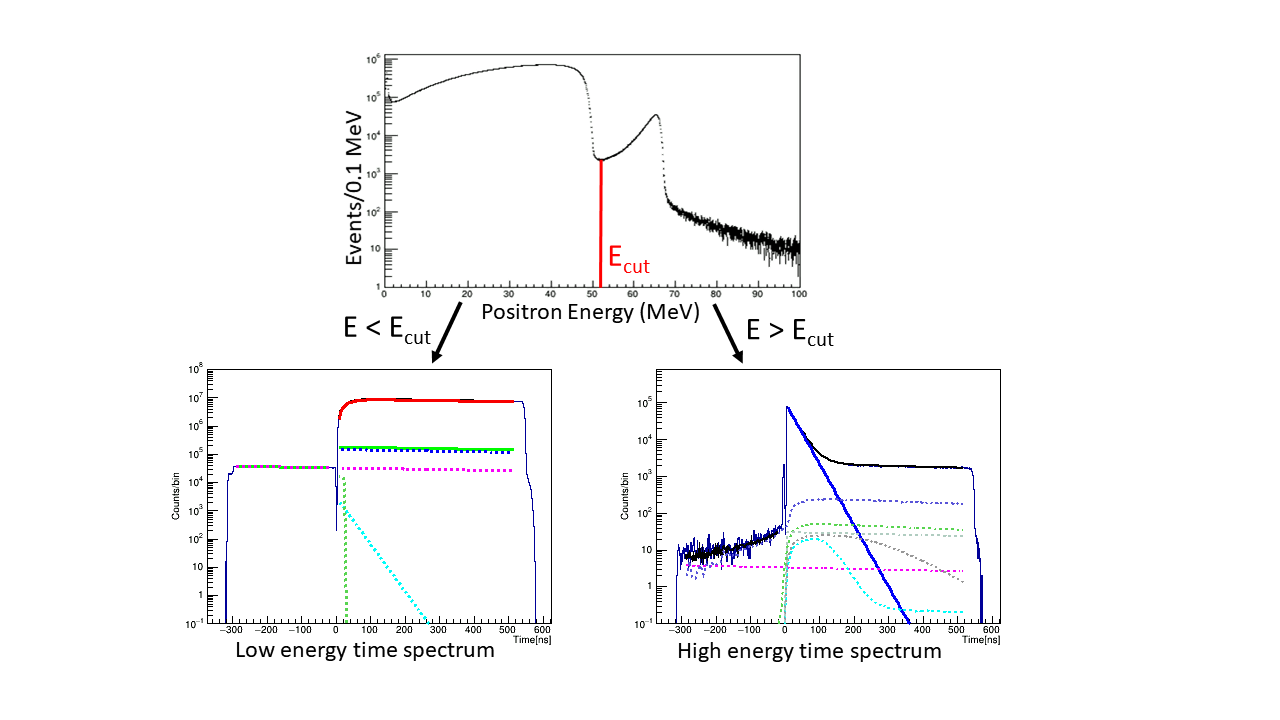
\includegraphics[scale=0.5]{sections/figures/Analysis.png}
\caption{The upper panel shows the positron energy spectrum with the red line indicating $E_{cut}$. The lower panels show the time distributions for events below and above $E_{cut}$. The black histograms are data, the red curve is the $\pi^+ \to \mu^+ \to e^+$ signal, and the blue line is the $\pi^+ \to e^+ \nu$ signal. The other histograms in various colors are the background terms.}
\label{fig:analysis}
\end{figure}

As mentioned before, several factors contributed to the size of the low energy tail, the most significant correction to the raw branching ratio. In addition to the finite energy resolution of the calorimeter and the presence of radiative decays, the positrons can lose energy on their way out of the target and before reaching the calorimeter in the non-instrumented parts of the detectors. 
%There was energy loss for positrons as they left the target and traversed material upstream of the calorimeter.  
Bhabha scattering upstream of the calorimeter can contribute to the low energy tail as well; due to the limited geometrical acceptance, secondary particles are often not absorbed by the calorimeter.  Electromagnetic showers are reasonably well contained for forward angles, but shower leakage increases at larger angles due to the reduced amount of calorimeter material.  The challenge of understanding and modeling these effects contributes to the low energy tail being the dominant source of systematic uncertainty.
%to the low energy tail in an imperfect detector means that the low-energy tail of the measured positron energy spectrum for PIENU events is the largest source of systematic uncertainty.

PIENU took special measurements to understand the response of the calorimeter, by injecting 70 MeV beam positrons into the detector at various angles. The response was highly non-uniform as a function of the angle between the positron track and the calorimeter axis; at small angles the low-energy tail was very small, but at large ($>45^\circ$) angles, it grew quickly. 
The measured energy spectrum with a beam of positrons injected along the NaI crystal axis and into the centre of the crystal, is shown in Figure~\ref{fig:0degrees_data} which displays significant bump features due to photo-nuclear effects. The details of the spectrum are discussed in \cite{Aguilar-Arevalo5}; the most important parameter is the percentage of the spectrum extending below $E_{cut}$, which in the spectrum shown is about 0.5\%. By contrast, the tail correction used in the branching ratio analysis is about 3\%, due to the effects mentioned above. A calorimeter with a similar or greater number of radiation lengths to that of the PIENU calorimeter, but covering close to the full solid angle, would not suffer from many of these effects, leading to a significant reduction in the tail correction and uncertainty.

\begin{figure}[h!]
\centering
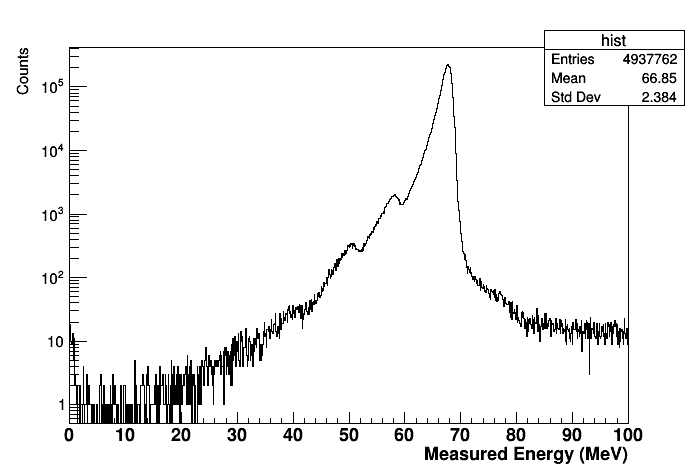
\includegraphics[scale=0.3]{sections/figures/0degrees_BINACsI.png}
%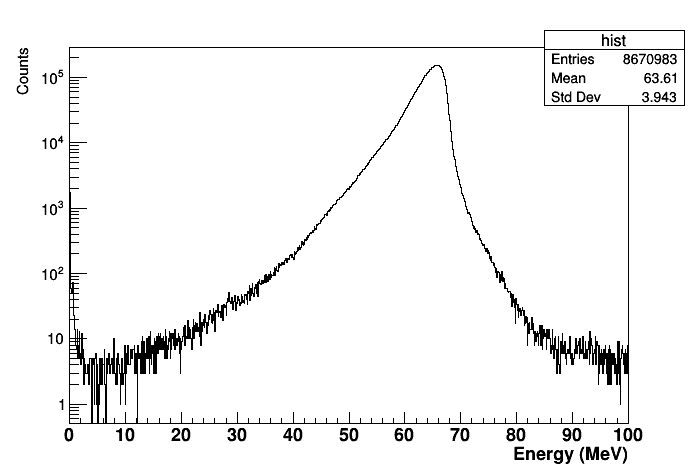
\includegraphics[scale=0.3]{sections/figures/48degrees_BINACsI.png}
\caption{Measured energy spectrum of a 70 MeV positron beam.}
\label{fig:0degrees_data}
\end{figure}

Pileup was another important source of systematic uncertainty. The usual pileup due to multiple beam particles was not severe at the relatively low beam rate of $\sim 50KHz$, and ensuring only one stopping pion at a time involved straightforward cuts in the data analysis. The much more serious pileup was a consequence of the long muon lifetime, coupled with the slow response time of the NaI(Tl) crystal. About 1\% of the muons stopped in the target lived longer than ten $\mu$s, and the long pulse width ($\sim\mu$s) of the NaI crystal raised the probability that positrons produced by such ``old muon" decays deposited energy overlapping with $\pi^+ \rightarrow \mu^+ \rightarrow e^+$ events. Such events are a background in the high-energy time spectrum, and stringent selection cuts, removing more than half the data, were employed to suppress them.  Also, ``neutral pileup" primarily from the environmental background of neutrons added energy to the calorimeter and boosted $\pi^+ \rightarrow \mu^+ \rightarrow e^+$ events into the high energy region.

The analysis of the full PIENU data set is  ongoing. A table of estimated uncertainties from  ~\cite{Aguilar-Arevalo3} is shown in Table~\ref{syst_table}.  To reach a precision of 0.01\%  all systematic effects would have to be addressed and reduced by a factor 3 to 10. The new detector concept detailed in section \ref{s:PIENUXEdet}
 addresses this challenge.  

\begin{table}[h!]
\centering
\caption{PIENU error table \cite{Aguilar-Arevalo3}.}
\label{syst_table}
\begin{tabular} {|c|c|}
\hline
Statistics & 0.19\% \\
Tail correction & 0.12\% \\
t$_0$ correction & 0.05\% \\
$\mu$ decay-in-flight correction & 0.05\% \\
Fitting parameters & 0.05\% \\
Selection cuts & 0.04\% \\
Acceptance correction & 0.03\% \\
\hline
Total & 0.25\% \\
\hline
\end{tabular}
\end{table}

 
 

%%\subsection{PiBeta-PEN}
%
The PiBeta
\cite{Pocanic5,Frlez2003vg,Pocanic4,Frlez2003pe,Bychkov2008ws} and
PEN \cite{Pocanic1,Pocanic2,Pocanic6} experiments shared much of the
same apparatus in a program of measurements focusing on the rare decays
$\pi^+ \to \pi^0 e^+ \nu(\gamma)$ (PiBeta), $\pi^+ \to e^+ \nu(\gamma)$
(PEN), and an exclusive radiative subset of the latter where the photon
was detected (both PiBeta and PEN).

The key components of the PiBeta/PEN apparatus were \cite{Frlez2003vg}:
\begin{itemize}
  \item a highly segmented (240 elements) spherical pure CsI crystal
    calorimeter covering $\sim 3\pi$\,sr of solid angle around
    the pion stopping target;

  \item a set of fast plastic scintillator beam detectors for time of
    flight (particle identification and momentum) measurement, energy
    degradation, and, ultimately stopping of pions (target detector);

  \item a pair of concentric cylindrical MWPCs surrounded by a thin
    20-bar plastic scintillator barrel, for identification, tracking and
    timing of particles traveling between the target and the CsI
    calorimeter; and

  \item for the PEN experiment only, a mini time projection chamber
    (mTPC) in front of the target for beam particle tracking
    \cite{Pocanic6}.
   
\end{itemize}

Both experiments were significantly constrained by systematical
uncertainties, especially the measurement of $R_{e/\mu}^{\pi}$ in PEN.
The key limitations were related to the imperfect separation of
$\pi_{\mu2}$ and $\pi_{e2}$ decays.  The primary culprit was the 12
radiation length thickness of the CsI calorimeter, which produced a
substantial low energy tail for 70\,MeV positrons (and photons)
extending well under the $\mu^+ \to e^+\nu\bar{\nu}$ continuous positron
energy spectrum.  Of similar significance were limitations on resolving 
the $\pi$, $\mu$, and $e$ pulses in the target, as well as some of the
critical background processes (various decays in flight, pileup).

%Controlling the above systematic uncertainty sources in a more ambitious,
%next generation of rare pion decay experiments will present a further
%significant challenge. 

Key strategies that proved effective in PiBeta
and PEN provide a useful foundation to build on for the proposed
measurements.
Beam and central tracking detectors need to be designed with as low mass
as possible, and with a minimum (or no) inactive material in the path of
particles.  In PiBeta, the high stopping rate ($\sim 10^6\ \pi^+$/s)
measurement of the pion beta decay, required the use of a segmented
target.  

%Higher target segmentation, or use of pixel trackers, will be
%more critical at the much higher rates of the ultimate
%$\pi_{e3(\gamma)}$ branching ratio measurement.
%Even with a much thicker electromagnetic calorimeter than the one used
%in PiBeta/PEN, the next generation experiments will require the ability
%to measure directly, and with sufficient precision, the low energy
%response ``tail'' of the $\sim 70$\,MeV positrons and photons in the
%calorimeter.
The calorimeter material shown in Fig.\ref{fig:PEN} and its design geometry were critical in terms
of several requirements: (a)  energy resolution (luminous and
highly uniform response throughout the volume), (b) fast timing
resolution, and (c) ability to handle high event rates.  While the
PiBeta calorimeter could have benefited from improvements in (a),
and would also have significantly benefited from an improvement in
timing resolution (b), the 240-element segmentation was adequate for the
highest stopping rates used. 
%A liquid Xe calorimeter of $\sim 30X_0$
%thickness would address points (a) and (b) very well, but care must be 
%devoted to the ability to separate piled-up showers in an extremely high
%stopping rate measurement.
The extremely low mass and near-absence of inactive material in the beam
and central tracking detectors were also critical for PEN.  
%The
%next generation of experiments place even greater demands on tracking
%resolution and speed, and introduce possible use of Si pixel trackers.
%Under those circumstances, maintaining low detector mass and minimizing
%passive material in particle paths become even greater challenges;
%nevertheless these goals must be pursued.

\begin{figure}[h!]
\centering
\vspace{-20mm}
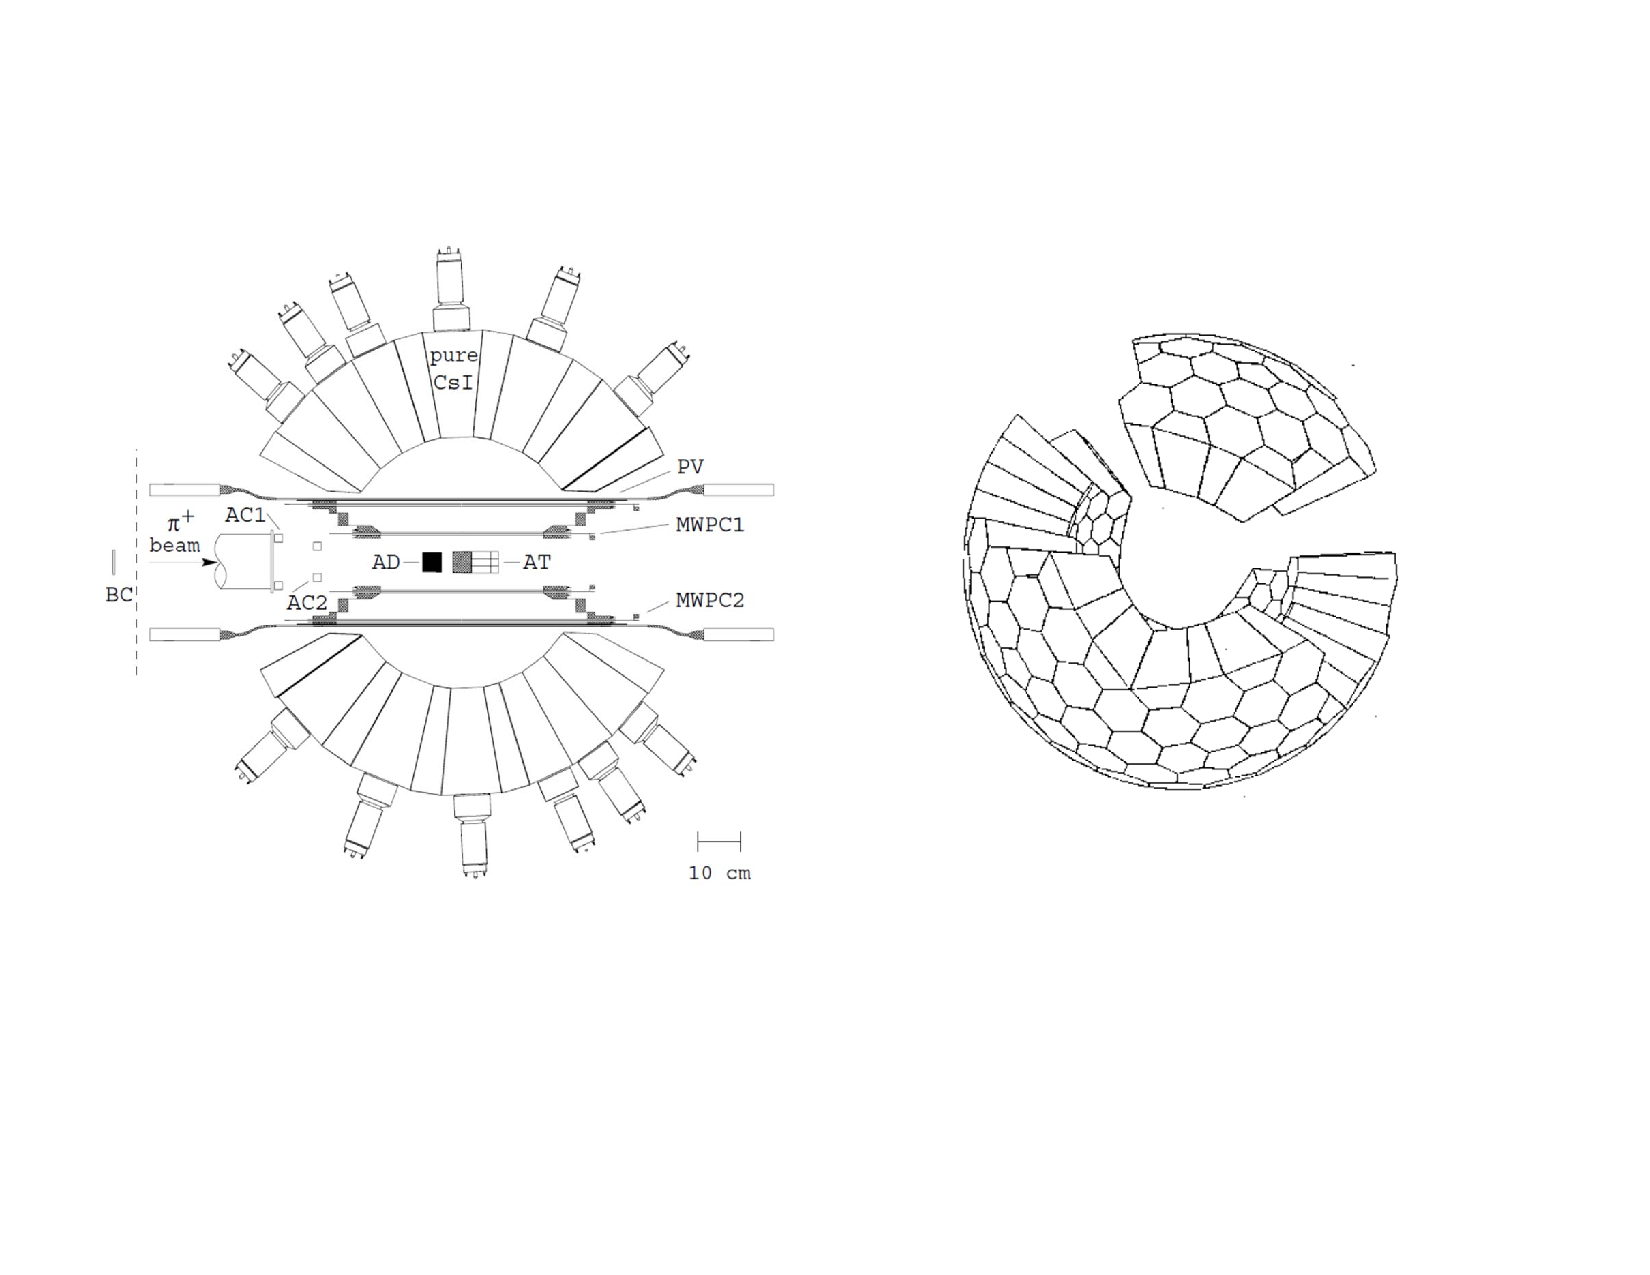
\includegraphics[scale=0.6]{sections/figures/PEN figure.pdf}
\vspace{-40mm}
\caption{Left: PEN detector. Right: Cutaway view of the PEN CsI crystal spectrometer\cite{Pocanic1,Pocanic2,Pocanic6}.}
\label{fig:PEN}
\end{figure}


%\subsection{Strategy and Goals}
\input{sections/Concepts/strategy.tex}
%\subsection{\nexp\ Strategy}

Precision frontier experiments require very high statistics as well as extensive evaluation of systematic uncertainties, backgrounds, biases and distortions in the data selection criteria. The two most recent pion decay experiments, TRIUMF PIENU and PSI PEN  provide highly insightful information on the  limitations of their techniques and the principal systematic effects which we have incorporated into our design concepts discussed below. These  measurements were performed using stopped pions that decay at rest either directly to a positron and a neutrino ($\pi^+ \rightarrow e^+ \nu$ decay) or first to a muon (and associated neutrino) that subsequently undergoes 3-body decay at rest in the target (decay chain $\pi^+ \rightarrow \mu^+ \rightarrow e^+$).  The  energy and time characteristics of the positrons emerging from those two decays are very different, and thus can be used to distinguish the decay channels. By measuring the ratio of positrons detected from the two channels, many systematic effects (e.g. pion counting, solid angle acceptance, efficiency, etc.) cancel out to first order, aiding in reaching high precision.  Despite being  mono-energetic the positrons originating from $\pi^+ \rightarrow e^+ \nu$ decays have their energy distribution broadened due to finite energy resolution of the calorimeter, shower leakages of low energy photons from the sides and ends of the calorimeter as well as the presence of radiative decays. Those effects result in a low energy tail hidden under the Michel spectrum and lead to the main correction and largest source of systematic effects in the branching ratio measurement. In order to minimize the energy tail for a precise experiment, a high resolution,  high radiation-length, and high acceptance calorimeter must be chosen.  Other significant systematic effects are associated with pulse pile-up and decays-in-flight of pions prior to stopping in the target. To supress all these  small effects to the level $< 0.01\%$ we propose to use a highly segmented stopping target.

The new measurement of $R_{e/\mu}$ would build on the techniques refined in the previous
experiments with high energy resolution like TRIUMF PIENU and high acceptance for positrons and
gammas like PSI PEN. In addition, it would employ emerging technologies in 
highly granular 4-dimensional tracking in an active stopping target using low gain avalanche 
diode (LGAD) silicon detectors. The combination of these two features, tracking in a highly
segmented fast active target (ATAR) and a high acceptance fast electromagnetic calorimeter (CALO) promise
to reduce the systematic impact of key challenges in the earlier experiments.

In the following we focus on the $R_{e/\mu}$ aspect of the proposed program because the systematic
requirements for achieving O$(10^{-4})$ precision are very demanding. The pion beta decay experiment
would equally benefit from the fast response of both active target and calorimeter, but the 
target thickness will be increased to spread out the wider stopping range of the 
%foreseen $\sim$100 MeV/c
pion beam with 100-fold higher rate than required for the $\pi \rightarrow e(\mu)$ measurement. 


%\subsection{Statistics}

%It is estimated that $3 \times 10^8\; \pi^+ \rightarrow e^+ \nu$ %events can be collected in two years of operation, satisfying the %statistics goal. 

%In addition to improvements in the precision of the PIENU branching ratio, orders of magnitude improvements would be anticipated in sensitivity to sterile neutrinos in decays $\pi^+ \rightarrow e^+/\mu^+ \nu_H$ and to decays involving dark sector particles like $\pi^+ \rightarrow e^+/\mu^+ \nu \textrm{X}$ as mentioned in Sec. \ref{Exotics}.

%\todo{Statement for PiBeta}


\subsection{Active Target (ATAR)}
\begin{figure}[h!]
\centering
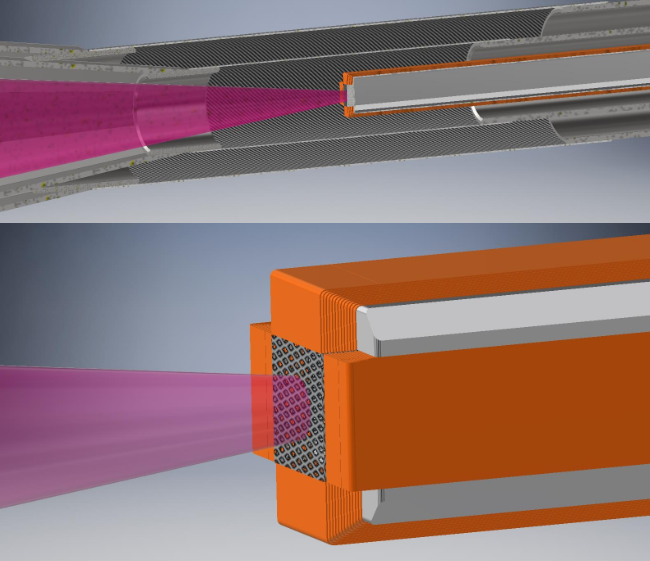
\includegraphics[scale=0.4]{sections/figures/atar1.png}
\caption{place holder: fig:atar1}
\label{fig:atar1}
\end{figure}

Fig.~\ref{fig:atar1} shows a concept drawing for  the pion beam entrance channel and  the active target. The  focused and collimated beam with a 1 cm diameter area passes through degrading plastic scintillators and two layers of double sided Si-strip detectors (not shown) before hitting the target. 
The stopping target (ATAR) is a rectangular prism of 20 mm transverse size and 5.76 mm in beam direction. It consists of 48 layers of AC LGAD sensors with a strip pitch of 200 $\mu m$. This results in 100 channels per layer and 4800 channels for the full detector. Consecutive layers are rotated by 90 degrees.

%Before describing the target (ATAR) in detail, let us recall its The target has the following functionalities:


\begin{itemize} 
\item 
Pion stops are identified. The expected stopping distributions are presented in fig.~\ref{fig:sim.stops}.
\begin{figure}[h!]
\centering
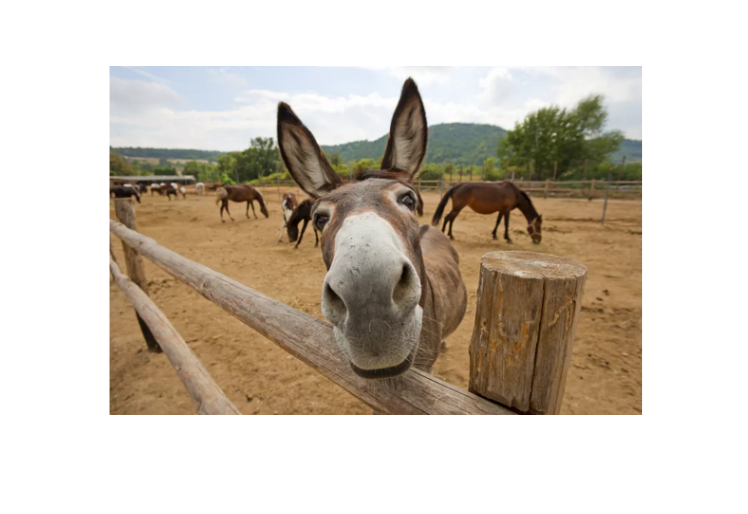
\includegraphics[scale=0.4]{sections/figures/ph.png}
\caption{place holder: fig:sim.stops}
\label{fig:sim.stops}
\end{figure}

\item
The $\pi \rightarrow \mu \rightarrow e$ Michel chain has to be suppressed by several orders of magnitude for measurement of the calorimeter energy response tail. The expected temporal pulse pair resolution of $dt\sim$1 ns provides a suppression factor of $\lambda_\pi dt=0.038$. An additional suppression results from a tight observation window of 
%several 
about one
pion lifetime, which disfavors the slower muon decay. Further separation is based on topology and energy 
deposition. Muons from pion decay have 4.1 MeV energy and a projected range of 0.8 mm in silicon. The $<$200 $\mu m$ segmentation of the detector was
chosen to resolve most tracks of isotropically emitted muons (see section~\ref{sec:simulation}). A zig-zag strip pattern will identify
the small fraction of muon tracks which stay within a layer and parallel to a strip. Fully depleted silicon detectors with minimal dead material
are essential to fully utilize the energy information. The required dynamic range of the readout is large as a pion can deposit 2 MeV in a
200 $\mu m$ range compared to 40 keV for a MIPS. \todo{MIPS number correct? Simone}

\item 
The "old" muons, accidental muons stops preceding the trigger signal, were a significant background in the previous generation of experiments by generating additional components in the time distributions
presented in fig.~\ref{fig:T1A}. In the PIENU experiment those were kept at an acceptable level, by imposing a wide pile-up window to -7 $\mu s$ before
the pion stop to let old muons decay, at the cost of 60\% of the statistics. For \nexp\, with its 
%5$\times$ 
higher beam rate, this is not 
%an option.
desirable.
Moreover the accidental rate will increase according to the increase of the beam rate. The much faster calorimeter will significantly reduce the pile-up contributions, which are more difficult to model and to determine correctly. In addition we will study how to reduce these accidentals by developing a local pileup rejection approach,
i.e. checking whether the observed decay electron belongs to the stopping vertex of the triggering pion.

\item
Muons arising from upstream pion decays are  relatively easily identified 
by their energy loss dE/dx properties and by  
kinks in their trajectories.
Pion decay
inside the target will be separated by kinks in the topology, dE/dx along the track, c.f. section~\ref{sec:simulation}, and range in the target. A sufficient Michel chain suppression and the tail suppression afforded by the 
%hermetic 
large acceptance
CALO will also allow  constraining a subtle background from Michel decays where the 4.1 MeV
 muon decays before leaving a track in the ATAR. 

\item
The ATAR will also be essential in defining event triggers. As will be discussed in section~\ref{section:daq}, the triggers will include
a relative simple CALO trigger based on all events above the Michel edge. An additional selective trigger based on fast ATAR tracking should suppress the $\pi-\mu-e$ sequence
to such extent, that the fully digitized ATAR information can be stored. The ultimate goal of this analysis is the offline suppression of Michel events so that the
low energy tail of the $\pi \rightarrow e \nu$ response can be measured in-situ. 

\end{itemize}



\todo{ATAR concept by Simone and Abe, please also sketch the readout. Need to address charge sharing. Peter sketched the ATAR readout in the DAQ section, as a starting point for Lawrence and Tim} 

While the LGAD ATAR design is the baseline option, we will also study a scintillating fiber option. Crossed planes of 250 $\mu m$ diameter
fibers should work well with the large signals expected. Recent developments in ultrafast fibers based on a new type of high performance nanostructured organosilicon luminophores (Kuraray NOL-11) and the  multi-channel  SiPM  array from  Hamamatsu  HPK  (S13552-HRQ) built for LHCb provide promising hardware components for this alternative.


\subsection{Calorimeter (CALO)}
\begin{figure}[h!]
\centering
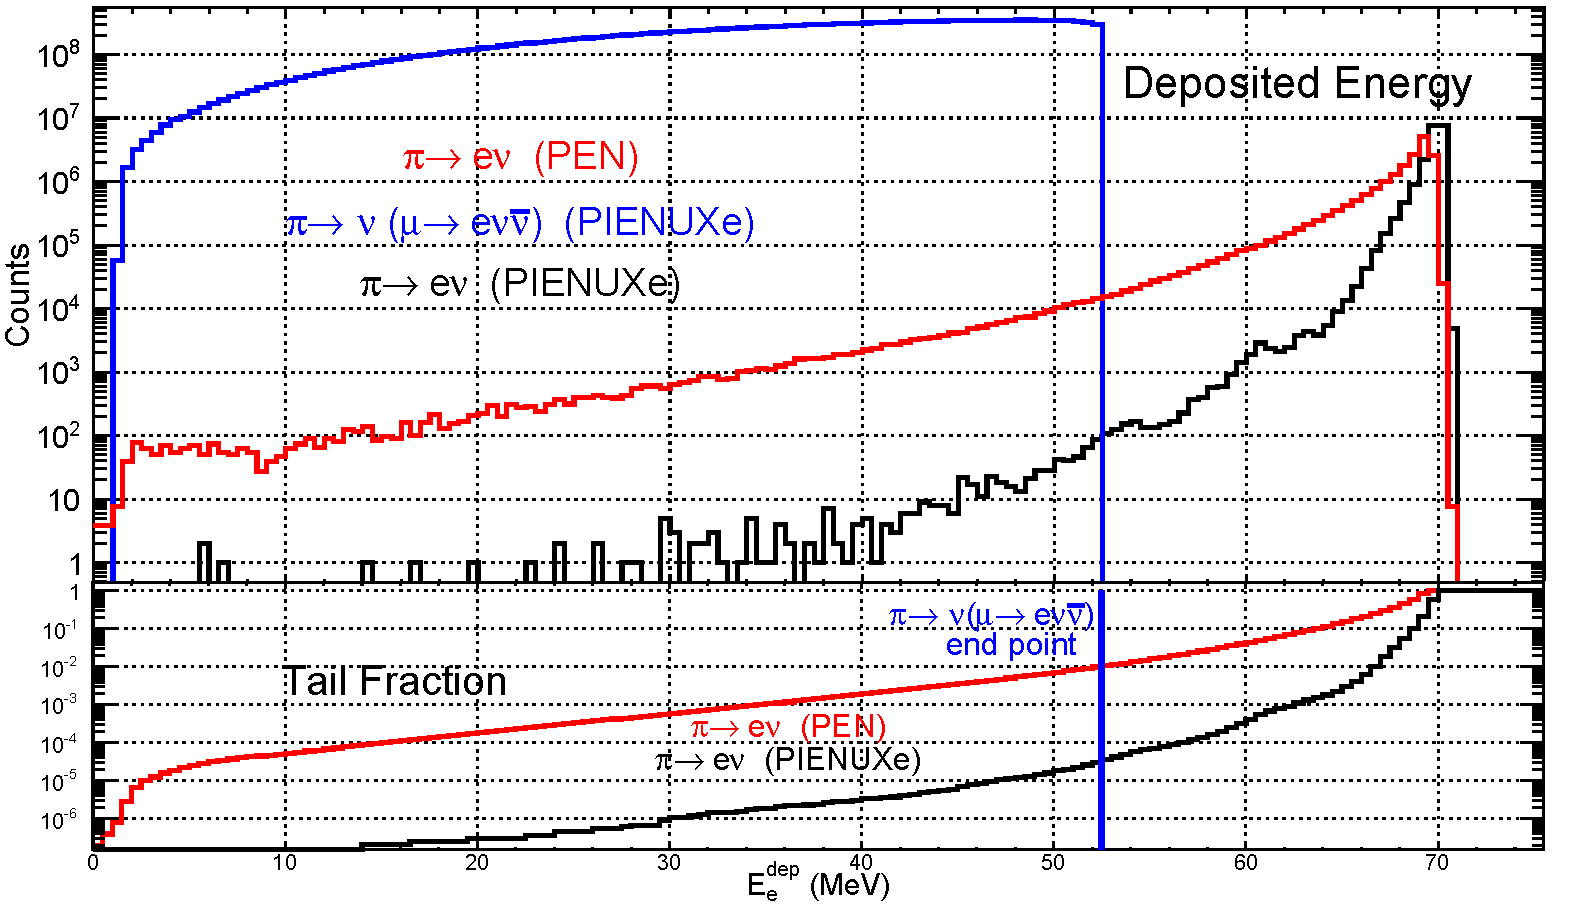
\includegraphics[scale=0.6]{sections/figures/tail.png}
\caption{Upper plot: histogram of $E_{e}^{dep}$, the $\pi_{e2}$ positron energy deposited in active components for a proposed 28 $X_{0}$ thick spherical LXe concept detector (black), compared with the same for the 12 $X_{0}$ pure CsI PEN apparatus (red), along with energy deposition
for the background $\pi \rightarrow \mu \rightarrow e$ decay chain events (blue).  Lower plot: comparison of the corresponding "tail" fractions as a function of $E_{e}^{dep}$; the LXe concept detector improves on the PEN fraction by two orders of magnitude in the region of interest.
\todo{I think we should add a PIENU spectrum as well and change the text accordingly}}
\label{fig:tail}
\end{figure}


A calorimeter covering 3$\pi$ solid angle with a thickness of 28 $X_0$ could dramatically reduce the ``tail” region
%-of-interest, 
which overlaps with the Michel spectrum, a key source of systematic uncertainty, see fig.\cite{fig:tail}. 
Two scintillation calorimeter options are presently under consideration: Liquid xenon and LSO crystals. Their main properties are compared in 
Table~\ref{tab:calos}. Evaluations  of potential energy and timing performance, rate capabilities, mechanical and cryogenic facilities, and cost are ongoing.
\begin{table}
\center
\begin{tabular}{cccccccc}
\hline
\hline
 detector 	&  density 		& 	dE/dx	&	$X_0$ 	& 	$R_M$ 	& decay time 	& $\lambda_{max}$ 	& light output  \\
 			&	g/cm3		&	MeV/cm	&	cm		&	cm		&	ns			&	nm				&	\%		\\	
\hline
LXe			&	2.953 		&	3.707	&	2.872	&	5.224	&	3, 27, 45	&	178			&	125 ?  \\
LSO(Ce)		&	7.40			&	9.6		&	1.14	&	2.07	&	40		&	402			&	85		\\	
\hline
\hline
\end{tabular}
\caption{LXe and LSO properties: density, minimum ioization, radiation length, Moli\`ere radius, decay times, maximum emission wavelength and relative light output compared to NaI(Tl). The LXe boiling point at 1 atm is 165.1 K. \todo{please check, LXe light output?}}
\label{tab:calos}
\end{table}


\subsubsection{LXe Calorimenter}
\begin{figure}[h!]
\centering
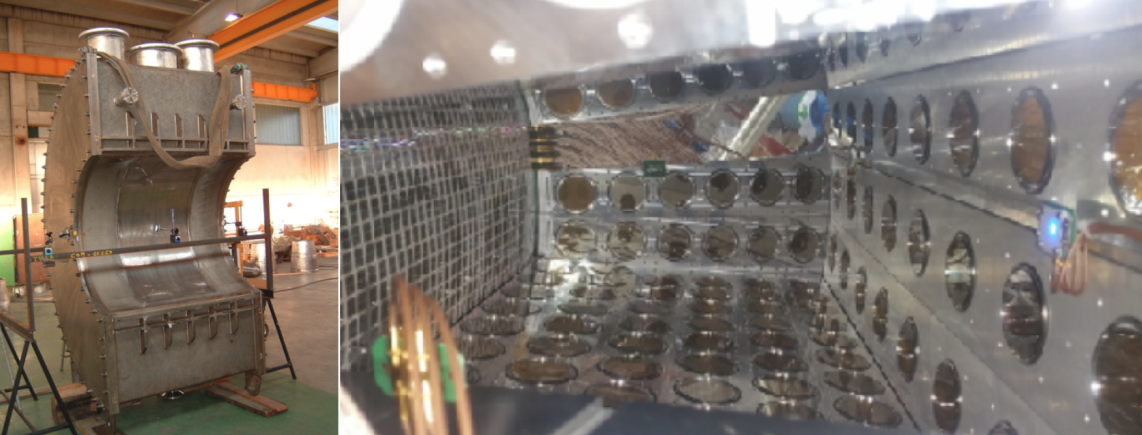
\includegraphics[scale=.4]{sections/figures/calo.meg.png}\vspace{3mm}\\
\caption{placeholder MEG, Toshiyuki please provide nice pictures}
\label{fig:calo.meg}
\end{figure}

One  concept for the new experiment is based on a liquid xenon (LXe) scintillating calorimeter for detection of positrons and gammas from pion decays. A 25-30 X$_o$ thick LXe scintillation calorimeter read out with fast-digitized SiPMs
has extraordinary properties including high light output (65k photons per MeV deposit), fast timing
($\sim$ ns decay time), and near complete containment of EM showers, making it suitable for this
application. Based on experience with the MEG LXe photon calorimeter \cite{Baldini} (see fig.~\cite{fig:calo.meg}) it is reasonable to
expect 1-2 \% energy resolution (comparable to \cite{Aguilar-Arevalo3} ), 50 ps timing resolution, and transverse (depth) position resolution of 5 mm 
(6 mm). Our Japanese collaborators are world experts on this detector technology. They have established basic LXe properties and suitable
simulation codes, conditioned on the MEG detector response, which will be critical for scaling up the design. \todo{Toshiyuki, Toshi, Sathoshi, that's just a placeholder for your part}
Due to the fast scintillation response of LXe (orders of magnitude faster than the NaI(Tl) and
pure CsI used in \cite{Aguilar-Arevalo1, Aguilar-Arevalo2} and \cite{Pocanic1, Pocanic2}), a low-energy pion beam rate of several 10$^5$ Hz can be used, more than an order of magnitude greater than previous experiments, which were impacted by pulse pile-up effects. Systematic effects would be reduced due to the highly uniform response and depth of the total absorption LXe calorimeter. 

\begin{figure}[h!]
\centering
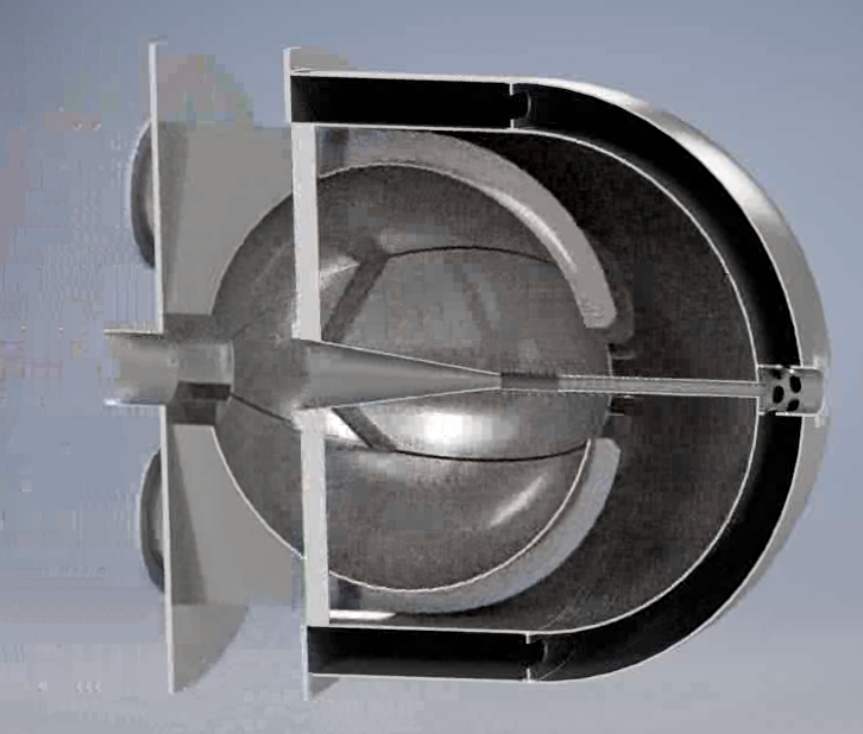
\includegraphics[scale=.4]{sections/figures/calo.Xe.png}
\caption{placeholder  \nexp\ CALO }
\label{fig:calo.Xe}
\end{figure}

\begin{table}
\center
\begin{tabular}{llll}
\hline
\hline
 parameter  &  	value		& 	unit		&  comment \\
\hline
Xe shell radius				&		&		&		\\
Xe volume					&		&		&		\\
Xe weight					&		&		&		\\
Xe entrance window radius	&		&		&		\\
vacuum window radius		&		&		&		\\
\hline
SiPM sensor size			&		&		&		\\
\# sensors					&		&		&		\\
\hline
\hline
\end{tabular}
\caption{Basic \nexp\ CALO parameters. \todo{Xe Ryan, SiPM Toshi, Satoshi et al}}
\label{tab:detpar}
\end{table}
The current conceptional design of the \nexp\ CALO draws on the experience of MEG, but involves several new features, see fig.~\ref{fig:calo.Xe} and Table~\ref{tab:detpar}.
\todo{Ryan: please continue}




\subsubsection{Crystal Calorimeter}


Another calorimeter concept is based on using LSO or LYSO crystals in a $3 \pi$ solid angle configuration similar to the PEN experiment discussed above. LSO has similar timing parameters to pure CsI (fast component aobut 45 ns) but much higher ligt output i.e. 75$\%$ of NaI(Tl). With a short radiation lenght about 1.1 cm, a compact calorimeter of 25-30 $X_0$ with excellent energy and time resolutions could be constructed. The same energy tail suppression would be realized as discussed above for the LXe option. The potential advantages of the crystal calorimeter approach include the absence of cryogenics and dead material, simpler mechanical facilities, and natural segmentation for handling high rates.

\subsection{Tracking}
\input {sections/Detector/tracking.tex}
\subsection{DAQ}
\input {sections/Detector/daq.tex}
\subsection{Simulations}
\label{sec:simulation}

\begin{figure}[h!]
\centering
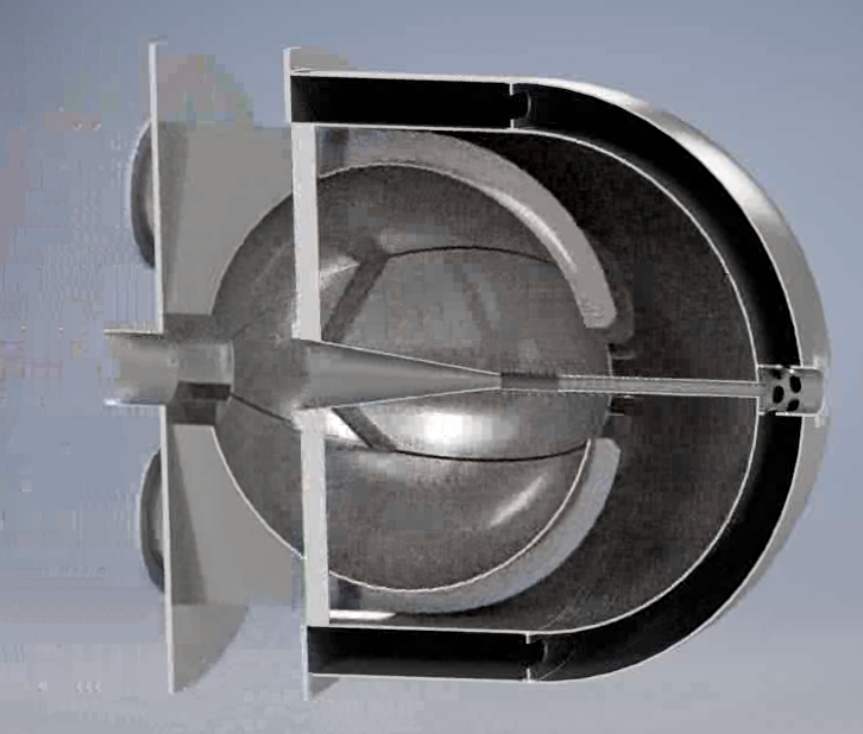
\includegraphics[width=.4\textwidth]{sections/figures/calo.Xe.png}
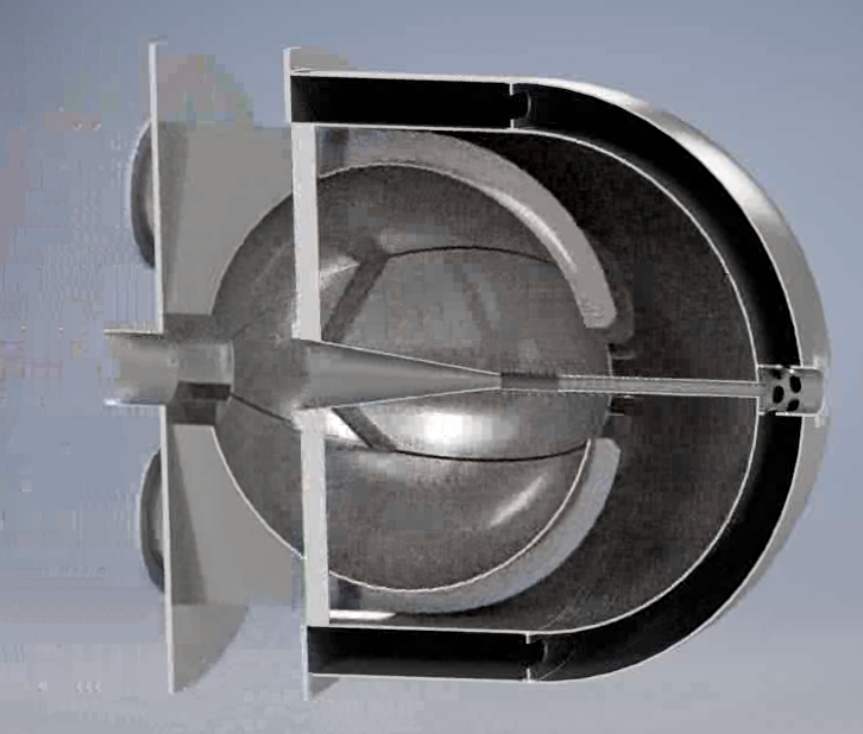
\includegraphics[width=.4\textwidth]{sections/figures/calo.Xe.png}
\caption{Left: A view of the active target system, showing the alternating planes. Right: A view of the full simulation,showing the calo }
\label{fig:simulation.view}
\end{figure}

A Monte Carlo simulation of the ATAR and CALO systems, based on the Geant4 simulation toolkit \cite{geant4}, has been undertaken in recent weeks. The simulated ATAR consists of 50 planes of 100 silicon strips, with the orientation of the strips within each plane rotated 90$^\circ$ with respect to its neighbours. Each strip has a $200 \mu m$ pitch and $120 \mu m$ thickness, giving our target an overall size of $20 mm \times 20 mm \times 6 mm$. Each strip can be read out separately in the simulation, allowing us to track particles as they move and decay within the target. A pure $\pi^{+}$ beam with a momentum spread of $72.84MeV \pm 0.01023$\% is situated upstream of the target. A degrader consisting of plastic scintillator is situated immediately upstream of the target, and its thickness of $7.5 mm$ was tuned such that beam pions are stopped in the center of the ATAR. Surrounding the ATAR and degrader is a carbon fiber beampipe, which acts as a low-Z window for positrons entering the CALO volume. The simulated volume of the CALO system consists of a $80 cm$ LXe sphere with a $17^{\circ}$ cone removed upstream of the ATAR for beam focusing and a $5 cm$ cylindrical cutout for the target and beampipe. Energy deposited in the CALO can be read out both through Geant4 truth information and by counting the scintillation photons which reach the outer radius of the detector.

Because of the lack of dead volume within the ATAR, as we can expect for AC-LGADs of this thickness, each particle leaves a distinctive track and energy signature. These signatures are not only useful for tagging decays of interest, but also supress our most common sources of background: decays in flight.
%\section{Previous Experiments}

\section{Beam and Beam Time}



 The first phase of the new experiment ($R_\pi$) would optimally need a beam with pion stopping rate of approximately $3\times 10^5$
  at momentum of $75$ MeV/c with $\frac{\Delta p}{p}=1\%$
in  a spot size  approximately 2 cm dia. This would result in $3\times 10^8$ $\pi^+\to e^+ \nu$ events for a 2-year run. For the $\pi^+ \to \pi^0 e^+ \nu$ experiment the  positive pion stop rate would have to be higher, $1-3\times 10^7$, possibly with  a larger momentum bite e.g. $\frac{\Delta p}{p}=3-5\%$ and using higher pion momentum. This would result in $\geq2\times 10^6$ $\pi^+ \to \pi^0 e^+ \nu$ events for a 4-year run. 

 At present there is only one existing TRIUMF beam possibility, M9A,  that could provide the necessary pion flux but it is apparently fully committed to the condensed matter program. A preliminary investigation of other possibilities was done independently by a TRIUMF technical panel\cite{PIBEAM}. Among the alternatives considered, the most attractive possibility appears to be provision of  a new pion production target (T1.5) and beam line (M13') at a location between the present T1 and T2 production targets as shown in fig.\ref{fig:T1A}. The estimated cost for providing these facilities was $\$8-10$M.
 
\begin{figure}[h!]
\centering
\vspace{-20mm}
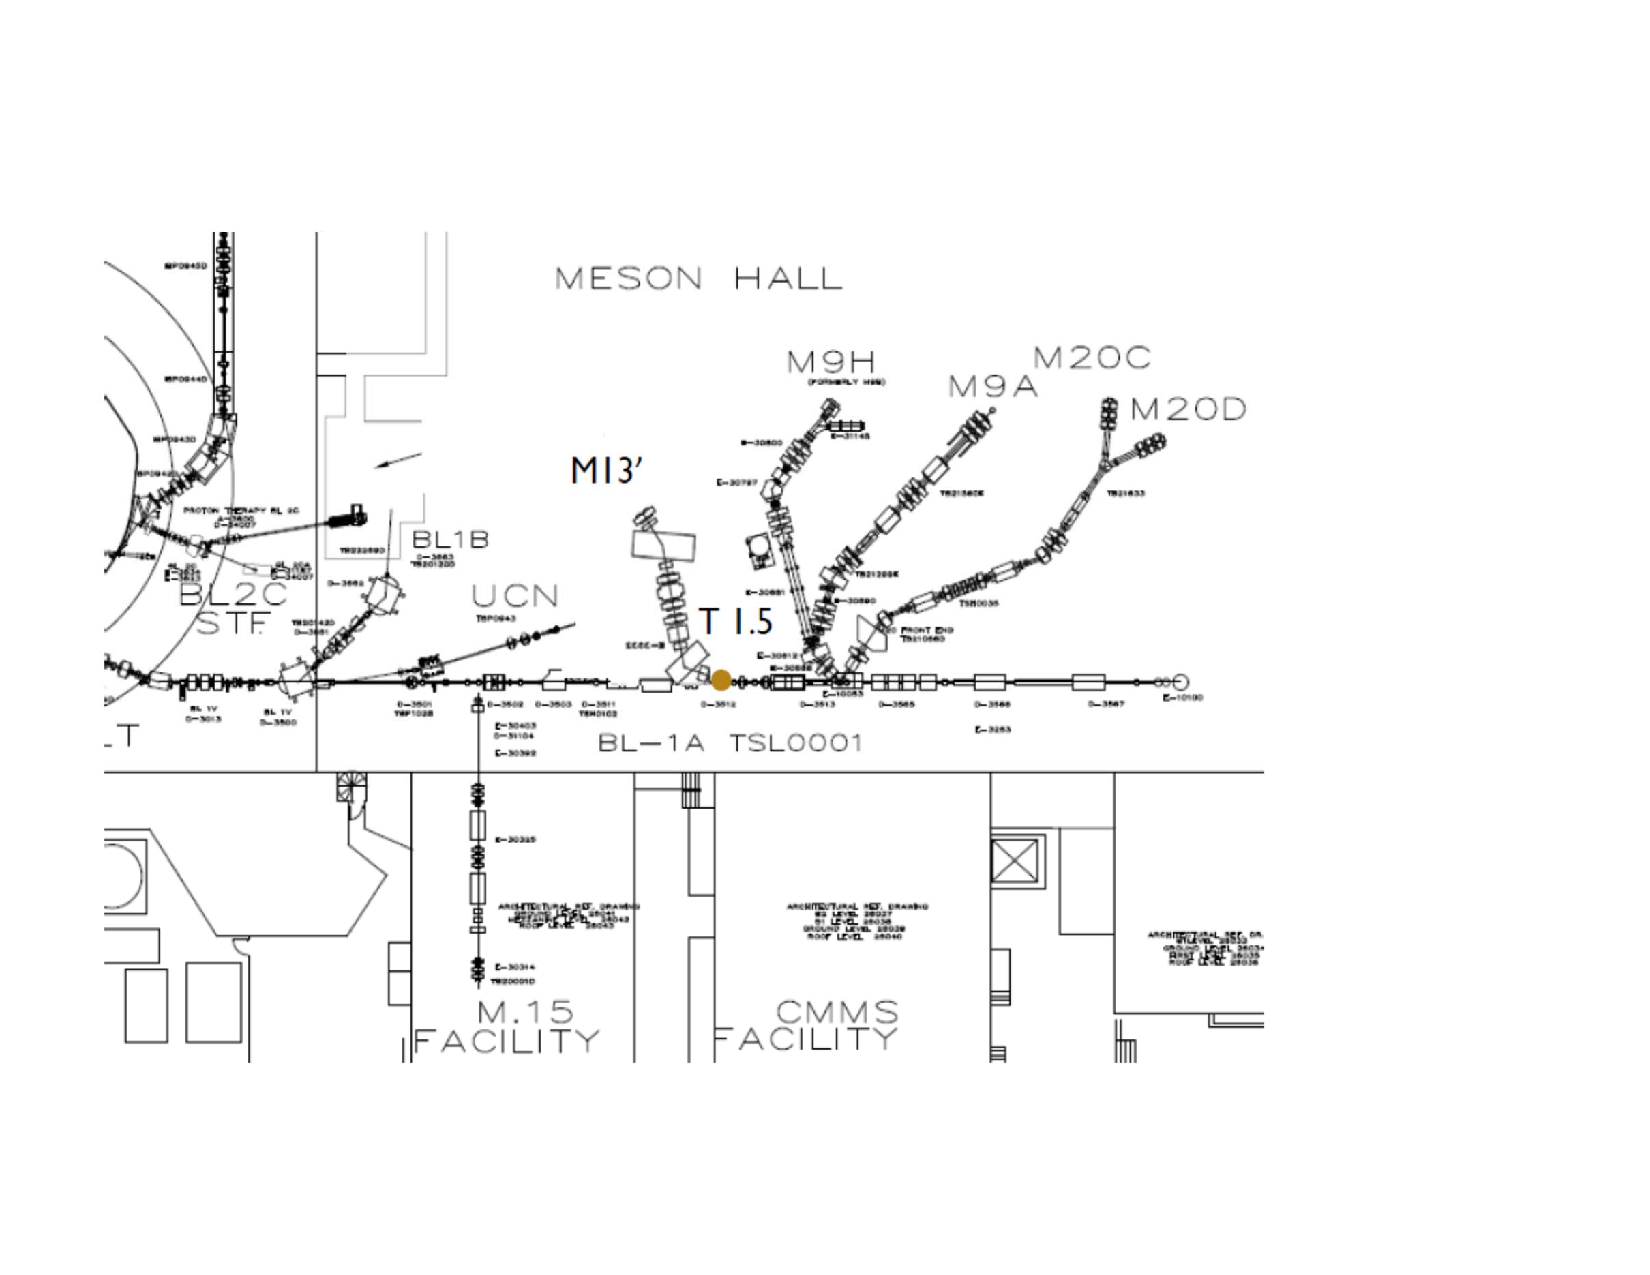
\includegraphics[scale=0.6]{sections/figures/T1.5M13'.pdf}
\vspace{-15mm}
\caption{Schematic concept for T1.5 and M13’, a short pion beam line in the current M11 area\cite{PIBEAM}}
\label{fig:T1A}
\end{figure}

The performance of a new M13' beam line may be estimated by considering a design like the PIE5\cite{PIE5} beam at PSI which has a solid angle acceptance of 150 msr, at 175 deg. take-off. Based on M13 flux measurements\cite{M13E}, it is estimated that a  pion flux of $\geq10^7/s$ could be obtained using a 4 cm thick Be production target. Such a beam line would meet the requirements of the new rare pion decay program discussed here and provide capabilities at TRIUMF for future  experiments involving positive and negative pions and muons. It would provide the highest fluxes at TRIUMF of surface muons for studies such as high precision Michel parameters, searches for $\mu \to e a$, muSR, and others.

\newpage
\section{Development Plan}
\subsection{R\&D}
Our R\&D plans over the next few years will proceed along five parallel tracks: 1) Beamline design; 2) Physics and detector simulations; 3) Active Target development; 4) Calorimetry; and, 5) Electronics/Triggering/DAQ.  Groups are formed and meeting regularly.  Small prototypes are planned where appropriate to evaluate detector components.  A test-beam program will be initiated for the Active Target and Calorimeter and any specialized beam line instrumentation to be developed.   We expect considerable involvement with TRIUMF Accelerator Division experts to design the needed new beamline.
\subsection{Timeline}
We present an optimistic calendar for the next five years.  We under the assumptions that all program approval stages and external funding decisions are positive and proceed without delay.  Naturally, the timeline is understood to be dependent on the actual pace of such decision milestones as well as any unforseen technical challenges.
\begin{itemize}
\item Spring/Summer 2021:  Refine simulations;  acquire small samples of testable equipment;  enlarge group
\item Fall 2021:  Develop full proposal; continue lab tests of devices; large-sample simulations
\item Winter 2022:  Submit proposal, begin to seek funding for new beamline and for large-scale prototype acquistions
\item CY 2023:  Begin beamline construction and carry out test beam campaign(s).
\item CY 2024: Begin beamline testing and evaluation;  full-scale production of detectors, electronics, DAQ subsytems
\item CY 2025: Begin data taking on \nexp
\item CY2026: Continue data taking, analysis, evaluation of equipment needed for pion beta decay phase
\end{itemize} 
\subsection{Collaboration}
The developing \nexp Collaboration is drawn from physicists having considerable experience in experimental precision physics, together with leading theorists who are carefully articulating the needed goals to maximize scientific impact.
%All of the experimentalists have significant experience in balancing statistical and systematic uncertainties, in careful modeling of the apparatus, and in the design of custom instrumentation.
%
Member groups led previous generation rare pion decay experiments -- {\tt PIENU, PEN} and {\tt PiBeta} -- and their collective experience is central to the design decisions that guide our emerging plans for a next-generation rare-pion-decay facility.
Key to this LOI and to the months of working meetings held to date, are ``Lessons Learned," from the TRIUMF and PSI experiences.
Other collaborators have worked on rare kaon decay experiments ({\tt BNL-E787/E949}) and on low-energy stopped muon experiments ({\tt MEG, MuLan, MuCap} and {\tt MuSun}); all have similar stringent beam and detector performance demands.
%
Many members of our team are involved in the Fermilab Muon $g-2$ experimental campaign, which has demonstrated the impact that can be made by using next-generation instrumentation and modeling tools to control systematics and acquire data at high rates.
Our collaboratioin has built both crystal and LXe calorimeters, various TPCs, a vast array of fast scintillating counters, custom arrays of waveform digitizers, fast DAQ systems, and beamline instrumentation.
Especially relevant are the experiences from our Japanese collaborators who developed the unique LXe calorimeter for {\tt MEG} and our UCSC collaborators who are  world leaders in LGAD development.
\subsection{Funding}
The support of proposal development and small prototypes is available among the research groups in our collaboration.  Our Japanese collaborators have received approximately \$100\,k
seed funding for developing an improved $R_{e/\mu}$ measurement and our UCSC group has support for LGAD development at the level we need at the moment.
Major funding for \nexp will be required for a new custom beamline at TRIUMF and for the detector and instrumentation package.
Following a successful experimental proposal defense, we  will approach NSERC to seek funds for a new low-energy pion/muon beamline for fundamental physics.
As advised by the TRIUMF Pre-Proposal Review Report (Feb 19, 2021), the new {\tt M13'} beam would cost $\approx 8-10$\,M\,CDN.

Detectors, electronics, and mechanical structures can be expected to cost as much or more than the beamline.  Given the anticipated costs of either a LXe or LYSO based calorimeter together with a finely instrumented Active Target, the appropriate U.S. funding possibilities include the NSF Mid-scale RI-1 program, which supports implementation projects in the cost range from \$6-20\,M.  Our collaboration has had several successful NSF MRI awards in the few \$M range that have delivered the custom instrumentation for the MuLan measurement of the muon lifetime and the Muon $g-2$ measurement of the muon magnetic anomaly.  The NSF is neatly cross-disciplinary and thus a nuclear / particle physics proposal can be successfully supported through the Mid-scale program.




%\section{Conclusions}
%\input{sections/conclusion.tex}


%\acknowledgments


\printbibliography
\end{document}
